
% !TEX TS-program = pdflatexmk
%\makeatletter\let\ifGm@compatii\relax\makeatother
\documentclass[pdftex,12pt,xcolor=pdftex,table]{beamer}
%\documentclass[handout,12pt,xcolor=pdftex,table]{beamer}
\synctex=1
\usepackage{comment}
\usepackage{etex}
\usepackage{amsmath}
\usepackage{amsthm}
\usepackage{amsfonts}
\usepackage{amssymb}
\usepackage{latexsym}
\usepackage{mathtools}
\usepackage[english]{babel}
\usepackage[utf8]{inputenc}
\usepackage{tikz}
\usetikzlibrary{calc,matrix,shapes,arrows}
\usepgflibrary{shapes.arrows}
\usepackage[nomessages]{fp}% http://ctan.org/pkg/fp
\newcounter{mycols}

\usepackage[]{graphicx}
\usepackage[sort]{natbib}
\usepackage{bibentry}
\usepackage{booktabs}
\usepackage{layout}
\usepackage[justification=centering,figureposition=bottom]{caption}
\usepackage{longtable}
\usepackage{lscape}
\usepackage{rotating}
\usepackage[figtopcap,center,scriptsize]{subfigure}%[figtopcap]
\usepackage{appendix}
\usepackage{setspace}
\usepackage[multiple,stable]{footmisc}
\captionsetup[longtable]{width=.75\textwidth}

\DeclareGraphicsExtensions{.png,.pdf}
\DeclareTextFontCommand{\emph}{\bfseries}

%% THEOREMS -------------------------------------------------------
\newtheorem{thm}{Theorem}[section]
\newtheorem{cor}[thm]{Corollary}
\newtheorem{lem}[thm]{Lemma}
\newtheorem{prop}[thm]{Proposition}
\theoremstyle{definition}
\newtheorem{defn}[thm]{Definition}
\theoremstyle{remark}
\newtheorem{rem}[thm]{Remark}
\numberwithin{equation}{section}
%
%% MATH -----------------------------------------------------------
\newcommand{\set}[1]{\left\{#1\right\}}
\newcommand{\eps}{\varepsilon}
\newcommand{\To}{\longrightarrow}

\newcounter{panel}[table]
\renewcommand{\thepanel}{\Alph{panel}}
\newcommand{\mypanel}[1][]{\refstepcounter{panel}Panel \thepanel: \ #1}

\newenvironment{stepenumerate}{\begin{enumerate}[<+->]}{\end{enumerate}}
\newenvironment{stepitemize}{\begin{itemize}[<+->]}{\end{itemize} }
%\newenvironment{stepitemize}{\begin{itemize}}{\end{itemize} }
\newenvironment{stepenumeratewithalert}{\begin{enumerate}[<+-| alert@+>]}{\end{enumerate}}
\newenvironment{stepitemizewithalert}{\begin{itemize}[<+-| alert@+>]}{\end{itemize} }
\newtheorem{assumption}{Assumption}
\newtheorem{proposition}{Proposition}
\usetheme{CambridgeUS}
\setbeamertemplate{navigation symbols}{}
\numberwithin{figure}{section}

\makeatletter
\let\@@magyar@captionfix\relax
\makeatother


  \setbeamercovered{transparent}

\usepackage{multicol}


\tikzset{arrowcases/.style={matrix anchor=west,%
  nodes={anchor=base west,%
         name=arrc-\the\pgfmatrixcurrentrow-\the\pgfmatrixcurrentcolumn},%
  execute at begin cell=\node\bgroup\math\displaystyle,%
  execute at end cell=\endmath\egroup;,%
  ampersand replacement=\&}}

\def\beginarrowcases#1\endarrowcases{
\begin{tikzpicture}[baseline=(O)]
  \matrix [arrowcases] {
  #1
  };
  \coordinate (A) at (arrc-1-1.west);
  \coordinate (B) at (arrc-\the\pgfmatrixcurrentrow-1.west);
  \coordinate (start) at ($(A)!0.5!(B) - (5em,0)$);
  \foreach \nn in {1,...,\pgfmatrixcurrentrow} {
    \draw[double, -triangle 45,<->] ($(start)+(0,1.5em - \nn em)$) -- (arrc-\nn-1.west);
  };
  \coordinate (O) at ($(start)-(0,0.5ex)$);
  \node at (-1em,0) {};
\end{tikzpicture}}

\makeatother
\setbeamertemplate{footline}
{
  \leavevmode%
  \hbox{%
  \begin{beamercolorbox}[wd=.25\paperwidth,ht=2.25ex,dp=1ex,center]{author in head/foot}%
    \usebeamerfont{author in head/foot}\insertshortauthor
  \end{beamercolorbox}%
  \begin{beamercolorbox}[wd=.4\paperwidth,ht=2.25ex,dp=1ex,center]{title in head/foot}%
    \usebeamerfont{title in head/foot}\insertshorttitle
  \end{beamercolorbox}%
  \begin{beamercolorbox}[wd=.35\paperwidth,ht=2.25ex,dp=1ex,center]{date in head/foot}%
  \insertshortdate{}\hspace*{3ex}
    \insertframenumber{} / \inserttotalframenumber\hspace*{1ex}
  \end{beamercolorbox}}%
  \vskip0pt%
}


\makeatletter
\@addtoreset{subfigure}{figure}
\makeatother
\makeatletter \@addtoreset{subfigure}{framenumber} \makeatother

\begin{document}
\author[Manuel \& Aprendiendo]{JAIR EBRATT RINCON \& DANIEL ALEJANDRO DIAZ DURAN}
\title{THE RISE OF EUROPE: ATLANTIC TRADE, INSTITUTIONAL CHANGE AND ECONOMIC GROWTH}
\date{JUNE 18, 2020} 
\subtitle{PAPER PRESENTATION}
\logo{
\includegraphics[scale=0.2]{puj.png}}
\institute[UNMSM]{
	\inst{}
		PONTIFICIA UNIVERSIDAD JAVERIANA. FACULTAD DE CIENCIAS ECONOMICAS Y 
		ADMINISTRATIVAS.
		\vspace{2mm} 
		\\ECONOMIC GROWTH AND COMPARATIVE DEVELOPMENT\\
		
	
}

\AtBeginSection[]
{
	\begin{frame}<beamer>{Content}
		\tableofcontents[currentsection,currentsubsection]
	\end{frame}
}


	\begin{frame}
		\maketitle
	\end{frame}

	\begin{frame}{Content}
		\tableofcontents
	\end{frame}

	\section{Authors}
		\begin{frame}{Authors}
			\justifying
			\centering
			Daron Acemoglu (MIT)
			
			
\includegraphics[scale=0.6]{pp1.jpg}
		\end{frame}
		\begin{frame}{AUTHORS}
			\justifying
			\centering
			Simon Johnson (MIT)
			
			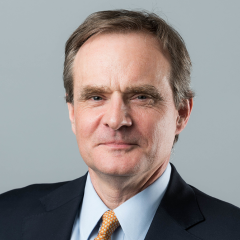
\includegraphics[scale=0.6]{pp2.png}
		\end{frame}
		\begin{frame}{AUTHORS}
			\justifying
			\centering
			James Robinson (Berkeley)
			
			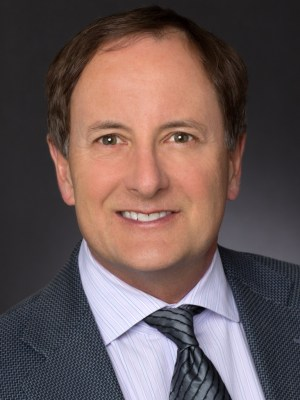
\includegraphics[scale=0.4]{pp3.jpg}
		\end{frame}
		
	
	\section{Introduction}
		\begin{frame}{Introduction}
			\justifying
			\begin{itemize}
			    \item Western Europe's accelerated growth since the 19th century.
			    \item “First great divergence ”since the 16th century.
			    \item Little consensus on the reasons for this growth and this divergence. 
			    \item Strong institutional differences between Western and Eastern Europe
			    \item Greater Atlantic trade by Western Europe.
			\end{itemize}
			\vspace{6mm} 
			\centering
			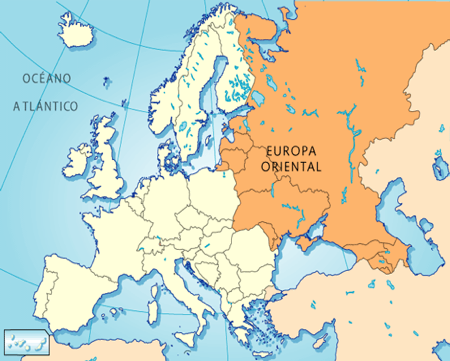
\includegraphics[width=4cm, height=3cm]{pp4.png}
			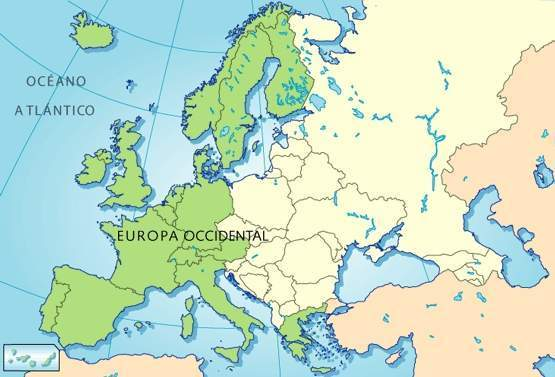
\includegraphics[width=4cm, height=3cm]{pp5.jpg}
		\end{frame}
		
	
	\section{Hypothesis}
		\begin{frame}{Hypothesis}
			\justifying
			    \begin{itemize}
			        \item Capitalist institutions are essential for incentives to undertake investment and for sustained economic growth, such as that experienced by Western Europe during the "First Great Divergence".
                    \vspace{7mm} 
			        \item Capitalist institutions are favored by commercial interests, especially new groups that do not receive commercial privileges from the state, but are not normally welcome by the monarchy, rulers, and elites.
	    		\end{itemize}
		\end{frame}
        \begin{frame}{Hypothesis}
		    \justifying
			    \begin{itemize}       
			        \item Institutions favored by economically and politically powerful groups are more likely to prevail.
                    \vspace{7mm} 
			        \item Atlantic trade and colonial activity created substantial opportunities for growth, enriching and strengthening commercial interests, including new groups with no ties to the monarchy.
			\end{itemize}
		\end{frame}
	
	\section{Data}
		\begin{frame}{Data}
			\justifying
			\begin{itemize}
			    \item European urban population of Bairoch, Batou and Cheve
			    \vspace{5mm} 
			    \item Madison'S GDP per capita estimates for 1500, 1600, 1700, 1820 and beyond.
			    \vspace{5mm} 
			    \item Bairoch, Batou and Cheve'S city-level data for Europe.
			\end{itemize}
		\end{frame}
		\begin{frame}{Data}
			\justifying
			\centering
			Urbanization rates weighted by population
			
			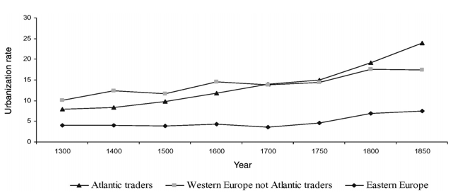
\includegraphics[scale=0.7]{pp10.png}
		\end{frame}
		\begin{frame}{Data}
			\justifying
			\centering
			GPD per capita from 1500 weighted population 
			
			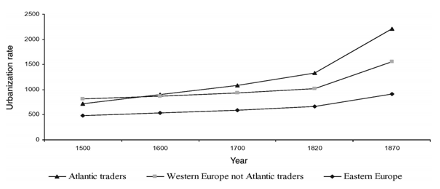
\includegraphics[scale=0.7]{pp11.png}
		\end{frame}
	
	\section{Model}
		\begin{frame}{Model}
			\justifying
			\centering
			\textit{$U_{jt} = d_{t} + \delta_{j} + \sum_{t\geq1600} \alpha_{t} \cdot WE_{j} \cdot d_{t} +\sum_{t\geq1500} \beta_t\cdot PAT_j \cdot d_t + X'_{jt}\cdot \gamma + \varepsilon_{jt}$} 
			\vspace{0mm} 
		    \begin{itemize}
		        \item \textit{$U_{jt}$} is urbanization (percentage of population in urban area) in country \textit{j} for time \textit{t}
		        \item \textit{$ WE_{j}$} dummy variable that indicates if the country is from Western Europe
		        \item \textit{$ d_{t}$}'s denote annual effects
                \item \textit{$ \delta_{j}$} denote country effects
		        \item \textit{$ X'_{jt}$} is a vector of other covariates
		        \item \textit{$ \varepsilon_{jt}$}is the term of error
		        \item \textit{$ PAT_{j}$} is an indicator for Atlantic merchant
		    \end{itemize}
		\end{frame}
	
	\section{Results}
		\begin{frame}{Results}
			\justifying
			\begin{itemize}
			    \item Western European urbanization grew by 6.9 percentage points relative to Eastern Europe between 1500 and 1850.
			    \vspace{11mm} 
			    \item Urbanization among Atlantic merchants grew approximately 8.5 percent more than in other western and eastern European nations.
			\end{itemize}
		\end{frame}	    
		\begin{frame}{Results}
			\justifying
			\begin{itemize}	    
			    
			    \item Protestant countries presented 4.6 more percentage points of urbanization and 30\% more of GDP in the period from 1500 to 1850.
			    \vspace{7mm} 
			    \item Inclusion of analysis of war processes
			    \vspace{7mm} 
			    \item Inclusion of analysis of hereditary influence of the Roman Empire
			\end{itemize}
		\end{frame}	

	\section{Justifying the Hypothesis}
		\begin{frame}{justifying the Hypothesis}
			\justifying
		    \begin{itemize}
			    \item Measure of "constrain on the executive". It measures the limitations on the use of power by the executive branch and is probably correlated with the security of merchants' property rights.
			    \vspace{4mm} 
			    \item Capital protection measure. This measure depends on the formal rights granted to urban merchants, particularly their protection in the event of a dispute with the nobility or the monarch.
			    \vspace{4mm} 
			    \item They were based on Langer (1972) and supplemented by stearns (2001)
			\end{itemize}
		\end{frame}
		\begin{frame}{justifying the Hypothesis}
			\justifying
		    \centering
		    \textit{$I_{jt} = d_{t} + \delta_{j} + \sum_{t\geq1600} \alpha_{t} \cdot WE_{j} \cdot d_{t} +\sum_{t\geq1500} \beta_t\cdot PAT_j \cdot d_t + X'_{jt}\cdot \gamma + \varepsilon_{jt}$}  
		    \begin{itemize}
			    \item \textit{$I_{jt}$} is our measure of institutions in country j at time t (restriction on the executive in the first part and protection for capital in the second part)
			    \vspace{4mm} 
			    \item Empirical results proved that there was a differential evaluation in institutions in Western Europe after 1500
			    \vspace{4mm} 
			    \item There is a close connection between Atlantic trade and the development of capitalist institutions
			\end{itemize}
		\end{frame}
		\begin{frame}{justifying the Hypothesis}
			\justifying
			\centering
			\scriptsize
			\textit{$$U_{jt}=d_{t} + \delta_{j} + \sum_{t\geq1600} \alpha_{t} \cdot WE_{j} \cdot d_{t} + \beta \cdot ln AT_{t} \cdot PAT_{j} + \sum_{t>1500} \gamma \cdot I_{j,1415} \cdot d_{t} + \eta \cdot lnAT_{t} \cdot PAT_{j} \cdot I_{j,1415} + \varepsilon_{jt}$$}
			\small
		     \begin{itemize}
			    \item\textit{$U_{jt}$} is the rate of urbanization
			    \item\textit{$AT_{t}$} is our measure of atlantic trade
			    \item\textit{$PAT_{j}$} is again an indicator for the potential Atlantic trader or the Atlantic coast-area ratio
			    \item\textit{j,1415} they are the "initial institutions of country j," The average of its institutions (executive restriction) in 1400 and 1500.
			    \item The terms \textit{$\gamma \cdot I_{j,1415} \cdot d_{t}$} allow any differential economic trend simply related to differences in initial institutions, which would apply without access to the Atlantic
			\end{itemize}
		\end{frame}	
		\begin{frame}{justifying the Hypothesis}
			\justifying
		    \centering
		    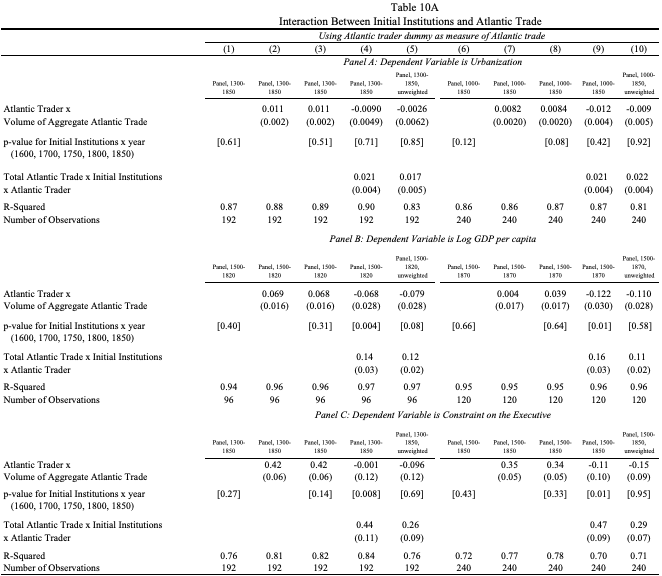
\includegraphics[scale=0.37]{pp12.png}
		\end{frame}
		\begin{frame}{justifying the Hypothesis}
			\justifying
		    \centering
		    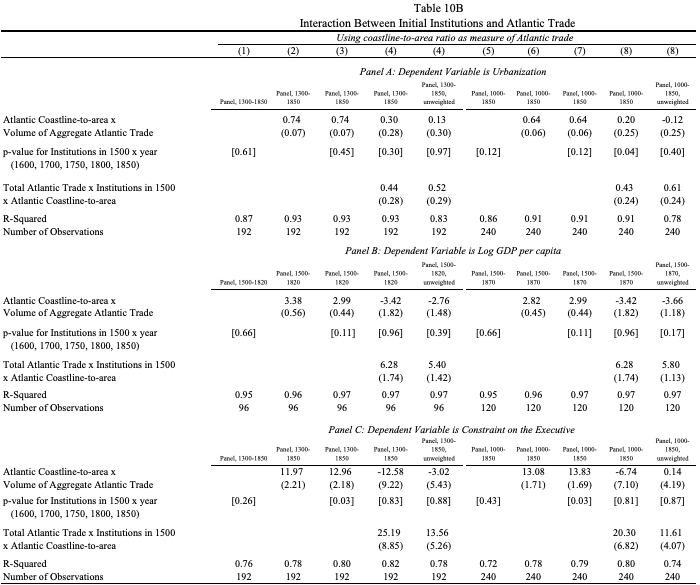
\includegraphics[scale=0.37]{pp13.png}
		\end{frame}
		\begin{frame}{justifying the Hypothesis}
			\justifying
		    \centering
		    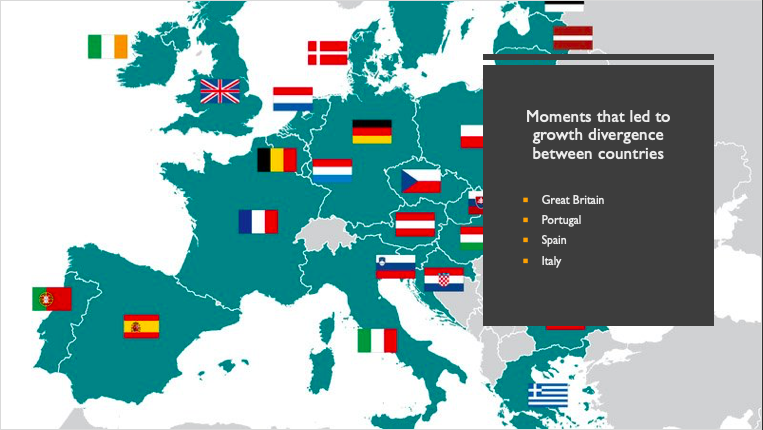
\includegraphics[scale=0.45]{pp16.png}
		\end{frame}
	
		\section{Contact Information}
		\begin{frame}{Contact Information}
			\justifying
			\begin{itemize}
			    \item jair.ebratt@javeriana.edu.co
			    \vspace{11mm} 
			    \item da-diaz@javeriana.edu.co
			\end{itemize}
		\end{frame}	    
		
\end{document}
